\section{Tests}

In our project we have developed tests after the fact.
This means that we started coding, making the features that we agreed on
and seeing if it works after they were developed.
In order to be certain that the quality is the same as before
and to ensure that we don't accidentally break something which wouldn't be on purpose.
If it works, then we would make tests to ensure that stability and robustness.
This is not the best way to do it, but it was the way we did it.
It also means that going forward and if it was a bigger project
we would ideally have to make tests before we started coding.
We have used the JavaScript test framework \textit{Mocha} for our tests.

\subsection{Unit tests}

Unit tests are tests that are made to test the smallest parts of the code.
In practice this will lead to making tests of small isolated functions and methods.
This is done to ensure that the code is working as intended and that it is robust.
With the \textit{Mocha} test framework, we have made unit tests for the backend and the OPC-UA client.
However, we have not made unit tests for the frontend.
This is because it is a user interface and it is not as easy to test, and as the frontend is not the main focus of the project, we decided to not make unit tests for it.
It also means that the frontend is not as robust as the backend and OPC-UA client, and is more likely to break if something is changed.
The unit tests for the backend are made to test the endpoints and the functions that are used in the endpoints.
The unit tests for the OPC-UA client are made to test the connection to the OPC-UA server and the functions that are used to both send and get data from the server. \newline

\subsection{Machine tests}
According to all the information we have gathered, we now need to find the optimal speed for each beer type. The speed we will find will be the optimal speed for brewing the beer, in your own home, in our case,
we would like the fail rate to be as low as posssbile, because our stakeholders are primarily hobbysit brewers, and would like the quality of the beer to be as good as possbile.
We have made a test for each beer type, where we have tested the speed of the machine, and the fail rate of the machine. The fail rate is the amount of times the machine fails to brew the beer.
And with all the data we have gathered, we have made a graph for each type to help us optimize the perfect speed for the machine. \newline
The way we gathered the data is was using our own brew function, where we could select thr beer type, beer amount aswell as the speed of the machine. On each test, we have different amount of beers brewed, this is because we only want the best fail rate possbile, and the amount of beers does not impact the fail rate only the machine speed does.
We made a graph of all the data gathered from the test, on the Y-axis we have the speed of the machine, and on the X-axis we have the fail rate. \newline

\subsubsection{Machine speed calculation}
From the data we have gathered from the tests, we made calculation for each individual beer type, and the graph made from the data, aswell as a failrate of 0.99, 
which leaves us with a 1\% fail rate. Now that we have all the numbers we need to calculate the optimal machine speeds for the brewing of each beer type. \newline
From the tendensy line of the graph, we got an equation that we can use to calculate the optimal speed for each beer type. The eqauation differentiates from each other the eqaution used is based on the line that is closets to the data points. which is where R2 is the closet to 1. which can be seen in each graph \newline
From the given equation, and the fail rate of 0.99, we can calcualte the optimal speed by setting 0.99 as the fail rate, and then solve for the speed. This is done by putting the fail rate into the equation, and solve each equation for the speed which is x value in each equation. \newline
This is done on each graph, and the results can be seen below in the following chapters of each beer type. \newline



\subsubsection{Pilsner}
For the Pilsner test, we have tested the machine with different speeds 600, 500, 400, 300, 200. And the amount of beers brewed for each test was 1000.

\begin{center}
    \centering
    \begin{figure}[H]
        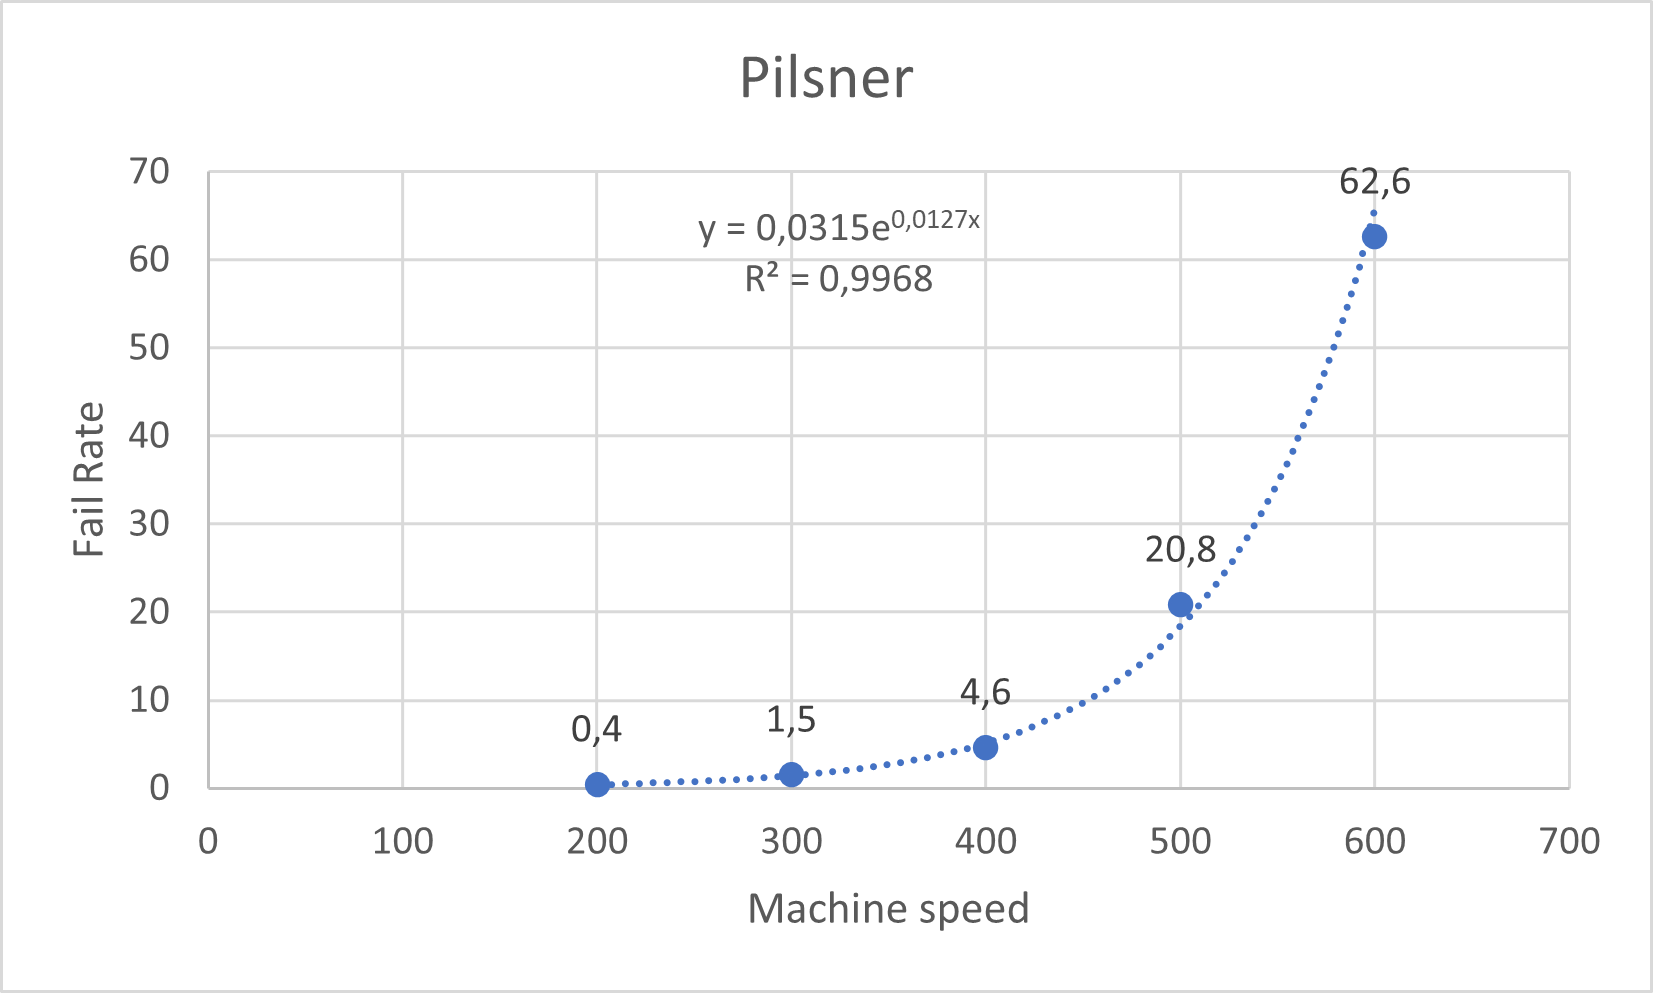
\includegraphics[width=1\textwidth]{img/Pilsner_graph.png}
        \caption{Graph over data from Pilsner tests}
        \label{fig:Pilsner_graph}
    \end{figure}
\end{center}

Figure \ref{fig:Pilsner_graph} shows the graph over the data from the Pilsner tests, with the R2 value and the equation for the line to find the optimal speed for the machine. \newline
From the calutaion made for Pilsner, we got the following machine speed after solving 263. This is the optimal speed for brewing pilsner for our hobbyist. \newline

\subsubsection{Wheat}
For the Wheat test, we used the following speeds, 300, 250, 200, 150, 100 and the amount of beers brewed for each test was 500.

\begin{center}
    \centering
    \begin{figure}[H]
        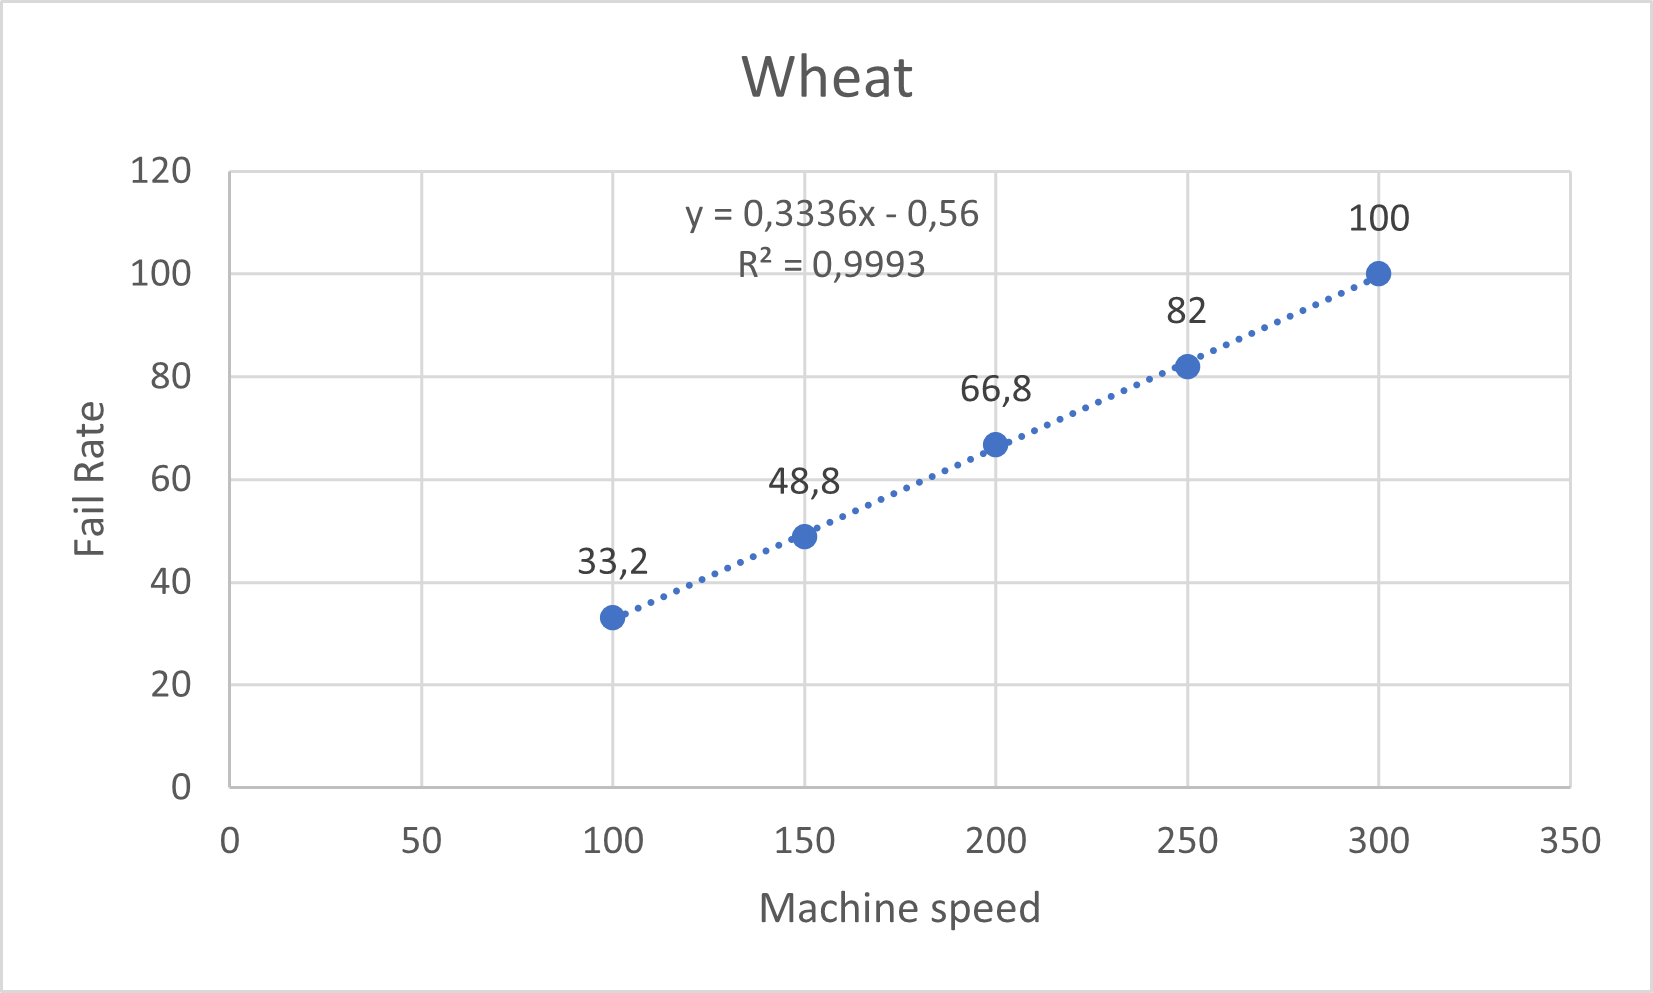
\includegraphics[width=1\textwidth]{img/Wheat_graph.png}
        \caption{Graph over data from Wheat tests}
        \label{fig:Wheat_graph}
    \end{figure}
\end{center}

Figure \ref{fig:Wheat_graph} shows the graph over the data from the Wheat tests, with the R2 value and the equation for the line to find the optimal speed for the machine. \newline
From the calutaion made for Wheat, we got the following machine speed after solving 5. This is the optimal speed for brewing Wheat for our hobbyist. \newline

\subsubsection{IPA}
For the IPA test, we used the following speeds, 150, 125, 100, 75, 50 and the amount of beers brewed for each test was 250.

\begin{center}
    \centering
    \begin{figure}[H]
        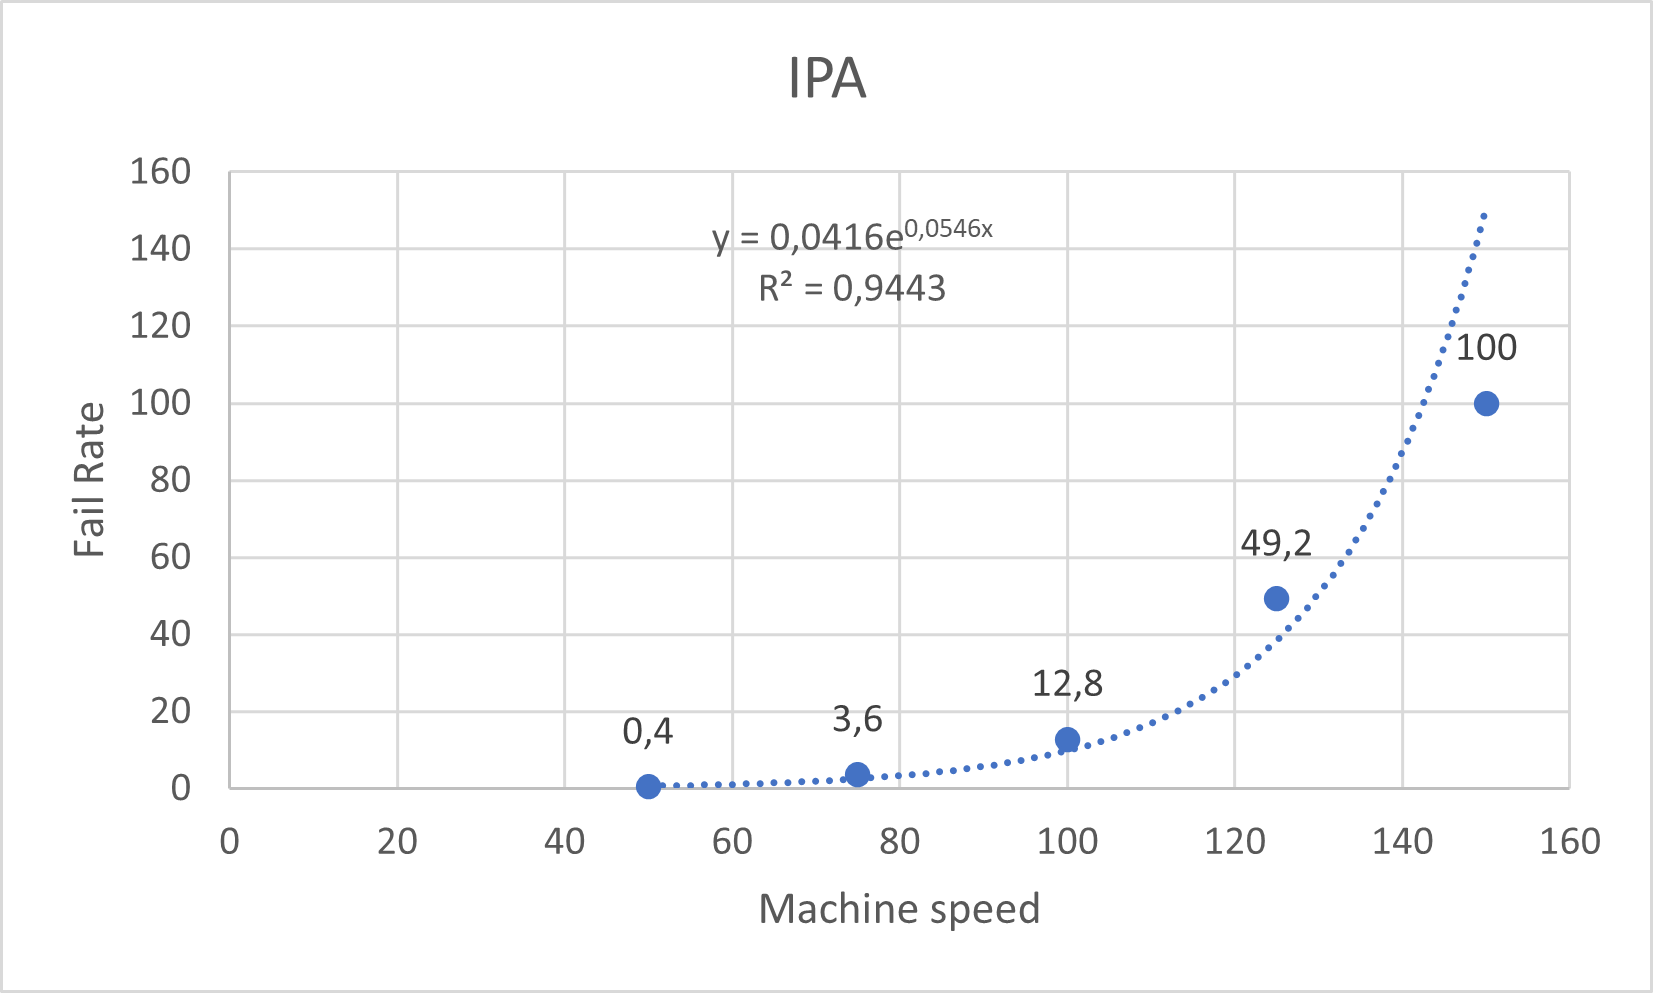
\includegraphics[width=1\textwidth]{img/IPA_graph.png}
        \caption{Graph over data from IPA tests}
        \label{fig:IPA_graph}
    \end{figure}
\end{center}

Figure \ref{fig:IPA_graph} shows the graph over the data from the IPA tests, with the R2 value and the equation for the line to find the optimal speed for the machine. \newline
From the calutaion made for IPA, we got the following machine speed after solving 58. This is the optimal speed for brewing IPA for our hobbyist. \newline

\subsubsection{Stout}
For the Stout test, we used the following speeds, 200, 175, 150, 125, 100 and the amount of beers brewed for each test was 300.

\begin{center}
    \centering
    \begin{figure}[H]
        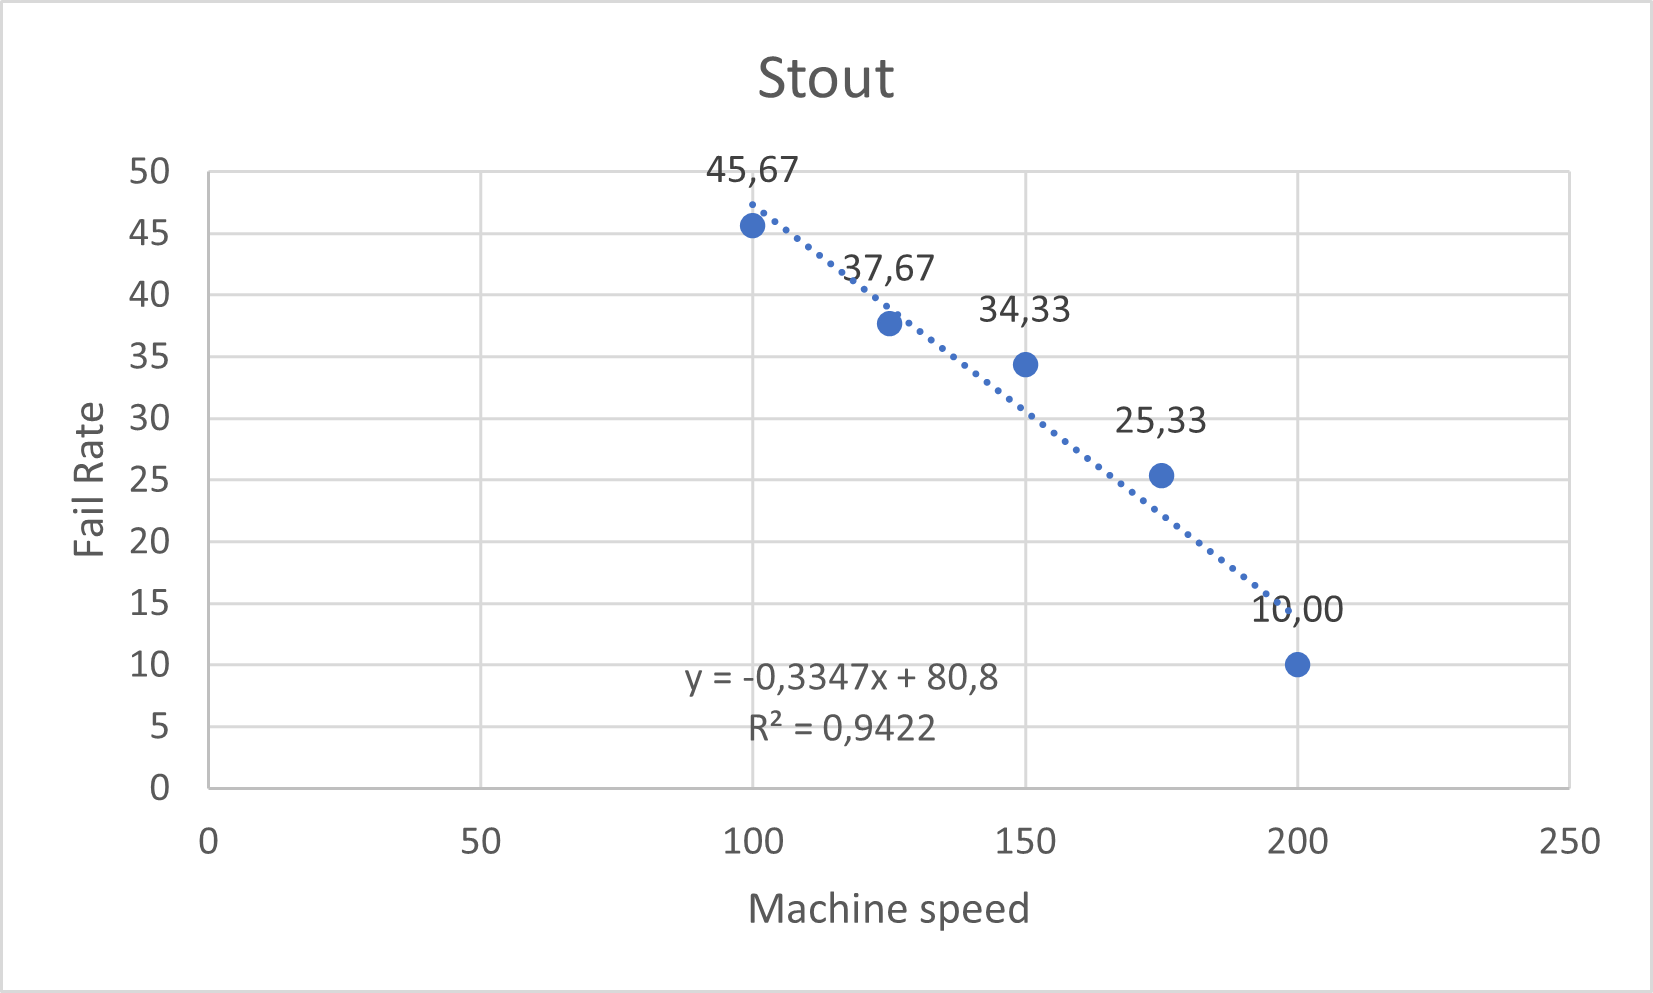
\includegraphics[width=1\textwidth]{img/Stout_graph.png}
        \caption{Graph over data from Stout tests}
        \label{fig:Stout_graph}
    \end{figure}
\end{center}

Figure \ref{fig:Stout_graph} shows the graph over the data from the Stout tests, with the R2 value and the equation for the line to find the optimal speed for the machine. \newline
From the calutaion made for Stout, we got the following machine speed after solving 238. This is theoretically the best machine speed for brewing Stout, but the problem is that the machine only allows the machine speed for Stout to be 200.
In our case the calulated machine speed is over the limit of the machine, this cant be done, because the macine will give us a failure, so if we want the hobbyist to have the lowest fail rate, as possbile, they need to brew Stout with a machine speed of 200, which is the maximum. \newline

\subsubsection{Ale}
For the Ale test, we used the following speeds, 100, 80, 60, 40, 20 and the amount of beers brewed for each test was 200.

\begin{center}
    \centering
    \begin{figure}[H]
        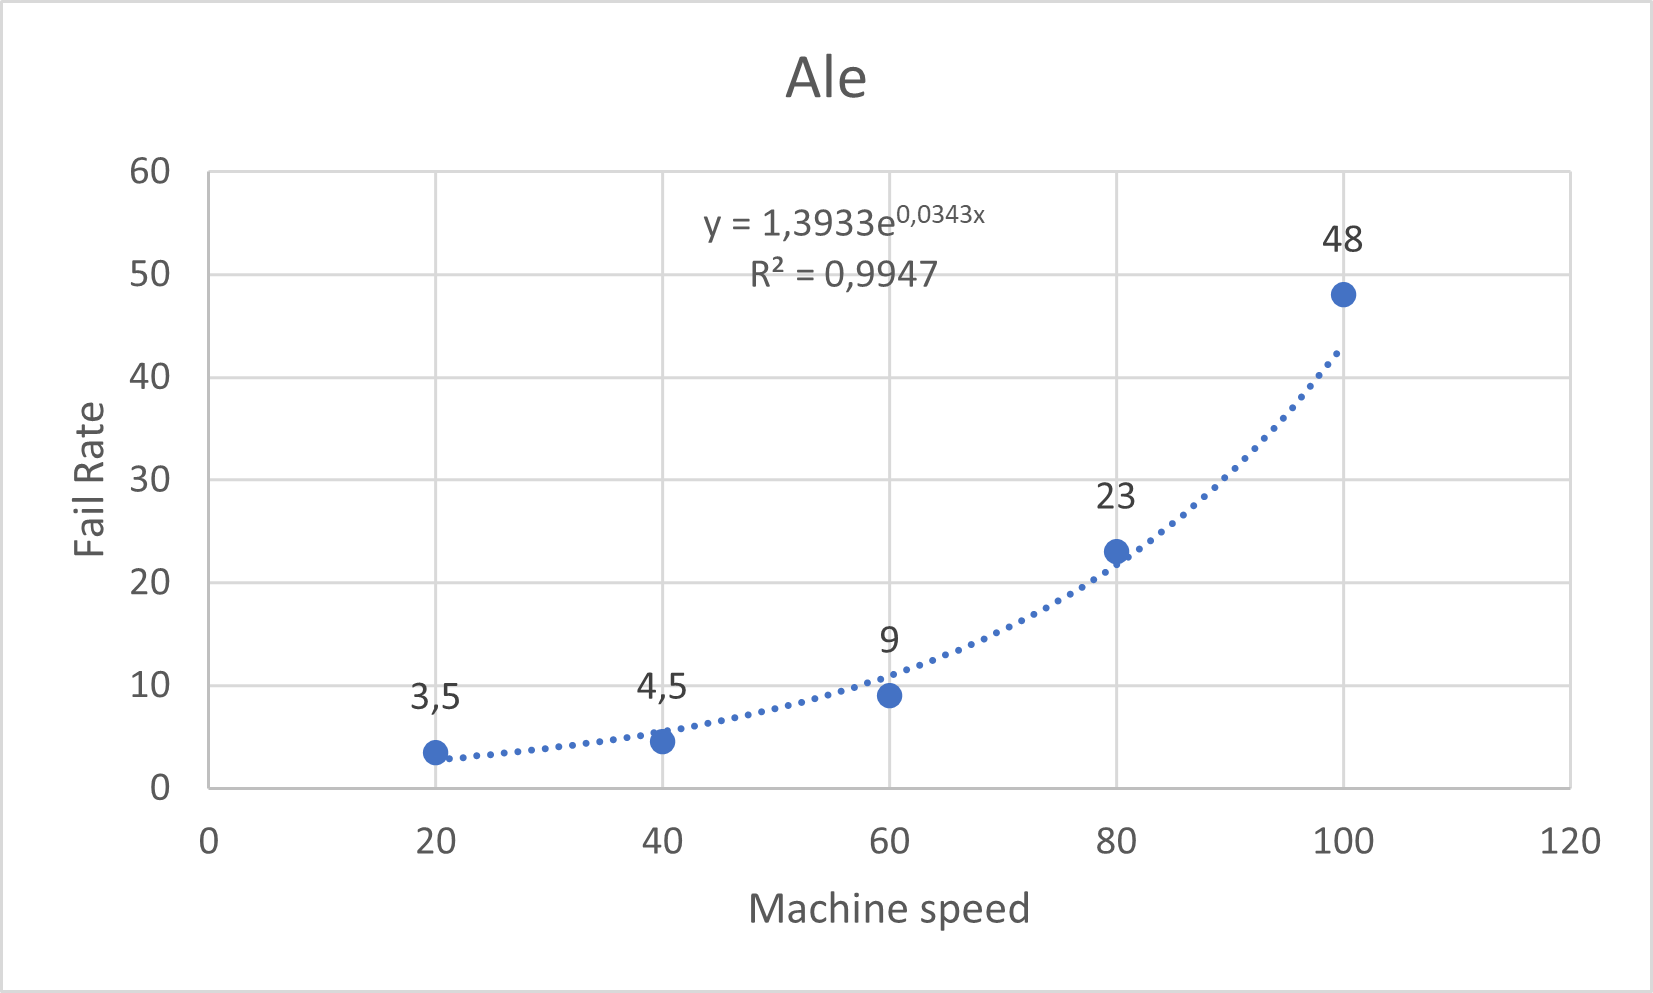
\includegraphics[width=1\textwidth]{img/Ale_graph.png}
        \caption{Graph over data from Ale tests}
        \label{fig:Ale_graph}
    \end{figure}
\end{center}

Figure \ref{fig:Ale_graph} shows the graph over the data from the Ale tests, with the R2 value and the equation for the line to find the optimal speed for the machine. \newline
From the calutaion made for Ale, we got the following machine speed after solving -10. This indicates the best speed for brewing Ale, but its not possibly to select this speed because it a negative value and the machine only allows for postive ones. 
So for our hobbysit to have the lowest fail rate as possbile, they would need to brew the Ale with a machine speed of 1, which is the slowest machine speed possbile, but would give the lowest fail rate. \newline


\subsubsection{Alcohol Free}
For the Alcohol Free test, we used the following speeds, 125, 100, 75, 50, 25 and the amount of beers brewed for each test was 225.

\begin{center}
    \centering
    \begin{figure}[H]
        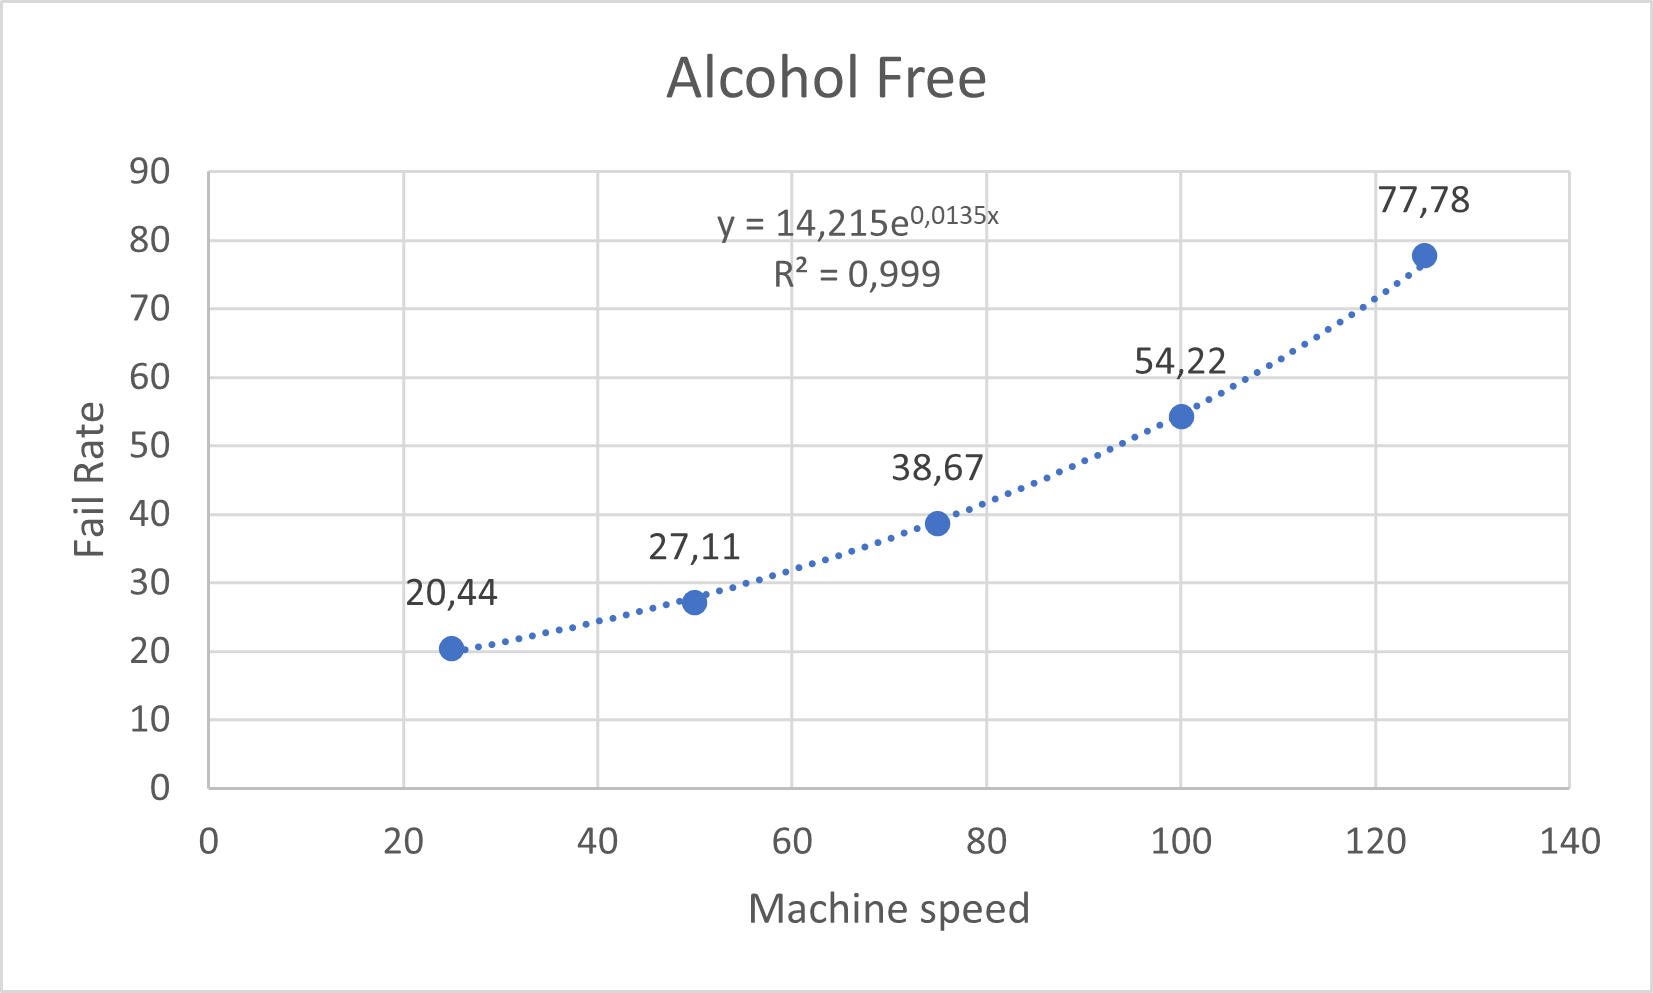
\includegraphics[width=1\textwidth]{img/AlcoholFree_graph.png}
        \caption{Graph over data from Alcohol Free tests}
        \label{fig:AlcoholFree_graph}
    \end{figure}
\end{center}

Figure \ref{fig:AlcoholFree_graph} shows the graph over the data from the Alcohol Free tests, with the R2 value and the equation for the line to find the optimal speed for the machine. \newline
From the calutaion made for Alcohol Free, we got the following machine speed after solving -198. Again we have a negative value so the best speed for brewing the Alcohol Free beer is 1. \newline